%
% logarithmus.tex -- slide template
%
% (c) 2021 Prof Dr Andreas Müller, OST Ostschweizer Fachhochschule
%
\bgroup
\begin{frame}[t]
\setlength{\abovedisplayskip}{5pt}
\setlength{\belowdisplayskip}{5pt}
\frametitle{Logarithmus}
\vspace{-20pt}
\begin{columns}[t,onlytextwidth]
\begin{column}{0.48\textwidth}
\begin{block}{Taylor-Reihe}
\begin{align*}
\frac{d}{dx}\log(1+x)
&= \frac{1}{1+x}
\\
\uncover<2->{
\Rightarrow\quad
\log (1+x)
&=
\int_0^x \frac{1}{1+t}\,dt}
\end{align*}
\begin{align*}
\uncover<3->{\frac{1}{1+t}
&=
1-t+t^2-t^3+\dots}
\\
\uncover<4->{\log(1+x)
&=\int_0^x
1-t+t^2-t^3+\dots
\,dt}
\\
&\only<5>{=
x-\frac{x^2}{2}  + \frac{x^3}{3} - \frac{x^4}4 + \dots}
\uncover<6->{=
\sum_{k=1}^\infty (-1)^{k-1}\frac{x^k}{k}}
\\
\uncover<7->{\log (I+A)
&=
\sum_{k=1}^\infty \frac{(-1)^{k-1}}{k}A^k}
\end{align*}
\end{block}
\end{column}
\begin{column}{0.48\textwidth}
\uncover<8->{%
\begin{block}{Konvergenzradius}
Polstelle bei $x=-1$
\(
\varrho =1
\)
\end{block}}
\vspace{-5pt}
\begin{block}{\uncover<9->{Alternative: Spektraltheorie}}
\uncover<9->{
Logarithmus $\log z$ in $\{z\in\mathbb{C}\;|\; \neg(\Re z\le 0\wedge\Im z=0)\}$
definiert:}
\vspace{-15pt}
\uncover<8->{
\begin{center}
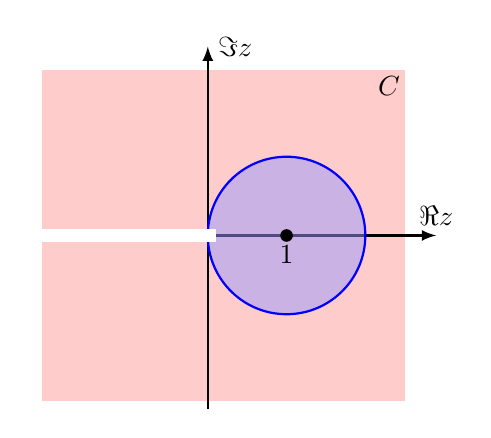
\begin{tikzpicture}[>=latex,thick]
\uncover<9->{
	\fill[color=red!20] (-2.1,-2.1) rectangle (2.5,2.1);
}
\draw[->] (-2.2,0) -- (2.9,0) coordinate[label={$\Re z$}];
\draw[->] (0,-2.2) -- (0,2.4) coordinate[label={right:$\Im z$}];
\fill[color=blue!40,opacity=0.5] (1,0) circle[radius=1];
\draw[color=blue] (1,0) circle[radius=1];
\uncover<9->{
	\draw[color=white,line width=5pt] (-2.2,0) -- (0.1,0);
}
\fill (1,0) circle[radius=0.08];
\node at (2.3,1.9) {$\mathbb{C}$};
\node at (1,0) [below] {$1$};
\end{tikzpicture}
\end{center}}
\end{block}
\end{column}
\end{columns}
\end{frame}
\egroup
